\documentclass[10pt, compress]{beamer}

\usetheme{m}

\usepackage{booktabs}
\usepackage{amsmath,amsfonts,amsthm,commath,bm}
\DeclareMathOperator*{\plim}{plim}

\title{Witty interesting title here}
\subtitle{}
\date{\today}
\author{Maxime and Angela}


\begin{document}
\maketitle

\begin{frame}[fragile]
    \frametitle{What is the Preprocessing problem?}
  
  \begin{center}
    \textbf{Preprocessing} constrains downstream data analysis, 
    
    particularly in \textbf{multiphase inference}:
  \end{center}
  
    \setbeamercovered{transparent}
    \begin{enumerate}[<+->]
    \item Original data is processed at each level of the analysis pipeline, often irreversibly, based on assumptions about what the future analysis may be and the observation mechanism
    \vspace*{5mm}
    \item Even if original data were passed down, many users may not know how to process the data themselves- the analyst performing the preprocessing may have detailed knowledge about the experimental situation
  \end{enumerate}
  
\end{frame}

\begin{frame}[fragile]
    \frametitle{The Multiphase Setup}

    Two phases:
    \begin{enumerate}
    \item \textbf{Preprocessing} = Data generation, collection, preprocessing
    \item \textbf{Downstream Analysis} = inference using output from phase 1
    \end{enumerate}
    
    \begin{figure}[h!]
    \centering
    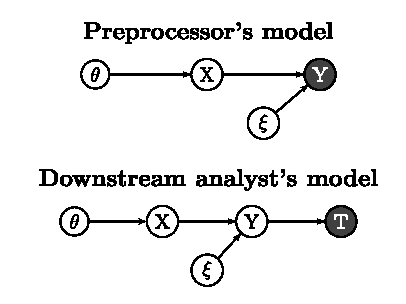
\includegraphics[width=.6\textwidth]{two_phase_setting.ps}
    \end{figure}

\end{frame}

\begin{frame}[fragile]
    Do we want another slide here? basic notation or definitions, discussion of the missingness and missingness pattern?

\end{frame}

\begin{frame}[fragile]
    \frametitle{NASA Raw Satellite Data}
    \begin{itemize}
        \item Data sent back to Earth is constrained by bandwidth
        \item $\rightarrow$ compression is necessary, but lossless compression is insufficient
        \item \textbf{Goal:} Valid science despite compression
    \end{itemize}
\end{frame}

\begin{frame}[fragile]
    \frametitle{High-throughput Biology: Expression Microarrays}
    
    \textbf{Raw data} = probe intensity measurements with control probes, but \textbf{want to study} log fold change in gene expression
    
    \textbf{Many levels of preprocessing:} 
    \setbeamercovered{transparent}

    \begin{enumerate} [<+->]
    \item \textbf{background correction} to reduce noise- many different algorithms, mostly passing down point estimates
    \vspace*{5mm}
    \item \textbf{normalization across different microarrays} to reduce systematic error- but can compromise inferential validity if data is used for other analyses
    \vspace*{5mm}
    \item data transformations, screening for data corruption, etc.
    \end{enumerate}
    
    At each step of preprocessing, large amounts of information are lost

\end{frame}

\begin{frame}[fragile]
    \frametitle{Regression}
    
    \textbf{Data:} $y_{ij} \sim N(\beta_0 + \beta_{1i}x_j, \sigma^2)$ for $j = 1 \ldots m$
    
    \textbf{Downstream analyst wants to estimate:} $\beta_0$ with $\beta_{1i}$ and $\sigma^2$ as nuisance parameters
    
    \textbf{Preprocessor reduces data to:} $T_i = \frac{1}{m}\sum\del{y_{ij} - \hat{\beta_{ij}}x_j}$ where $\hat{\beta_{1i}}$ is the OLS estimator.

\end{frame}

\begin{frame}[fragile]
    \frametitle{discussion of twitter example for people to think about}

 lots of data- approximately 8 tb a day if you include metadata and images (2010 estimate)
 what are some things downstream analysts would want to estimate, and what are some ways the original data could be compressed?
\end{frame}

\begin{frame}[fragile]
    \frametitle{What statistics should we retain?}
    

    \textbf{Optimal}- lossless compression to minimal sufficient statistics for a given research model
    
    This is only practical if there is an agreed-upon model. 
    
    \textbf{More reasonable}- hope downstream analyst's scientific model is related to researcher's observation model 

\end{frame}

\begin{frame}[fragile]

    other slides:
    another slide on what stuff to retain
    discussion of risk and regret
    discuss constraints of this work


\end{frame}

\end{document}
